%        File: hw1.tex
%     Created: Sat Apr 06 10:00 AM 2013 P
% Last Change: Sat Apr 06 10:00 AM 2013 P
%
\documentclass[11pt]{article}

\usepackage{amsmath, amssymb, amsthm, cite, graphicx, float, mathrsfs, commath, dsfont, bbm, bm}
\usepackage[mathscr]{eucal}
\usepackage[sc]{mathpazo}
\linespread{1.05}
%\usepackage{setspace}
%\onehalfspacing
\usepackage[margin=1in, top=.8in, left=.8in]{geometry}
\usepackage{color}

% new commands
\DeclareMathOperator*{\argmin}{arg\,min}
\DeclareMathOperator{\sgn}{sgn}
\newcommand{\E}{\mathrm{E}}
\newcommand{\Var}{\mathrm{Var}}
\newcommand{\Cov}{\mathrm{Cov}}
\newcommand{\Cor}{\mathrm{Cor}}
\newcommand{\id}{\operatorname{id}}
\newcommand{\diag}{\operatorname{diag}}
\newcommand{\Id}{\operatorname{Id}}
\newcommand{\tr}{\operatorname{tr}}
\newcommand{\Q}{\mathbb{Q}}
\newcommand{\C}{\mathbb{C}}
\newcommand{\R}{\mathbb{R}}
\newcommand{\Z}{\mathbb{Z}}
\newcommand{\F}{\mathbb{F}}
\newcommand{\N}{\mathbb{N}}

\newcommand{\indep}{\rotatebox[origin=c]{90}{$\models$}}

% 524 commands
%\newcommand{\norm}[1]{\| #1 \|}
\DeclareMathOperator{\spn}{span}
%\newcommand{\spn}{\operatorname{span}}
\newcommand{\onenorm}[1]{\| #1 \|_{L^1(\mathbb R^d)}}
\newcommand{\twonorm}[1]{\| #1 \|_{L^2(\mathbb R^d)}}

% 534 commands
\renewcommand{\Re}{\text{Re\,}}
\renewcommand{\Im}{\text{Im\,}}

\begin{document}
\pagestyle{empty}
\hfill Abraham Engle

\hfill Stat 571

\hfill \today
\begin{enumerate}
    %1
	\item 
		\begin{enumerate}
			\item I generated data from the mechanism $10^3$ times, each time using $n=10^3$ clusters. Histograms of the coefficient estimates from the GEE linear regression of $Y$ on $t$ and $X$ are
			\begin{figure}[H]
				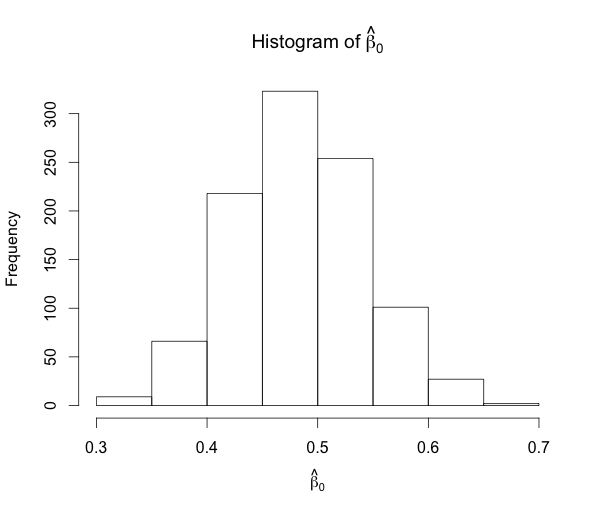
\includegraphics[scale=0.4]{Rplot1a0}
				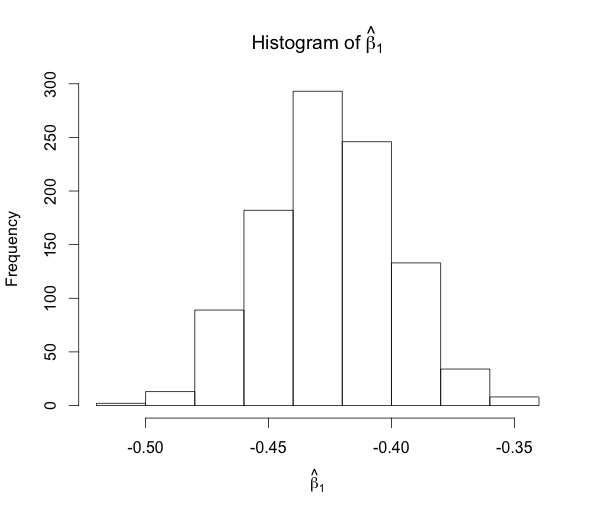
\includegraphics[scale=0.4]{Rplot1a1}
				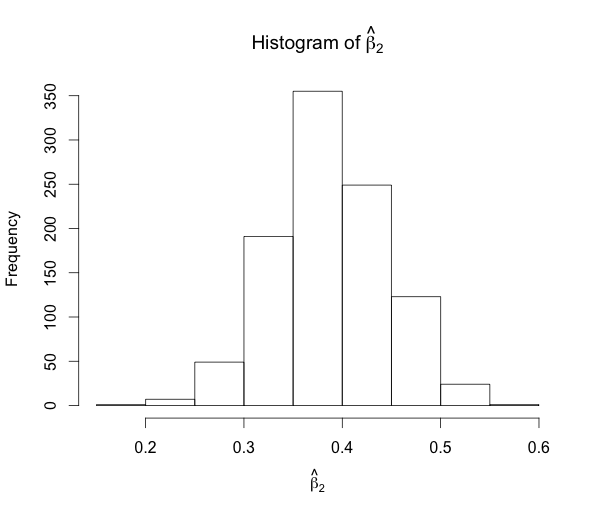
\includegraphics[scale=0.4]{Rplot1a2}
			\end{figure}
			and empirical coverage probabilities for the true parameters $\bm{\beta} = (1,-1,\frac{1}{2})$ are $0\%, 0\%$ and $48.5\%$. The histograms of the parameter estimates together with these coverage probabilities compared to the true parameters in the mechanism lead me to believe that complete case analysis for these data is not valid for inference. 
			\item The problem with this type of censoring is that the missingness depends on the outcome, so we should not hope for valid inference from complete case analysis. I graphed a spaghetti and a conditional plot from the data generating mechanism for 100 clusters:
			
				\begin{figure}[H]
					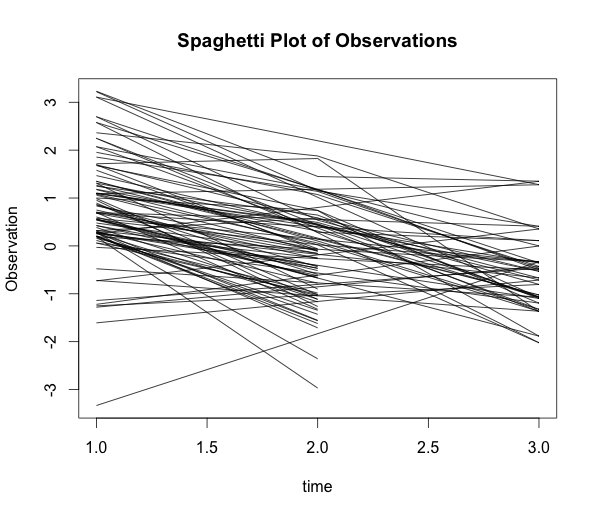
\includegraphics[scale=0.4]{Rplot1b3}
					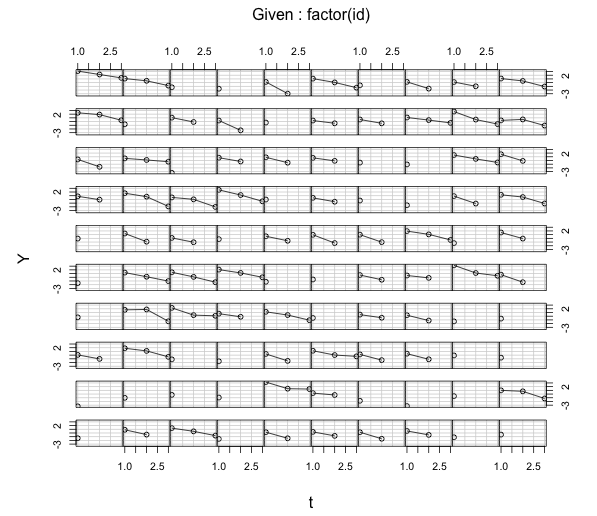
\includegraphics[scale=0.4]{Rplot1b4}
				\end{figure}
				the missingness is obviously very dependent on the outcomes.
			\\	For our given values of $\beta_0, \beta_1,$ and $\beta_2$ in the previous example, the marginal mean of observations is given by
				\begin{align*}
					E[Y_{it}|X_i] &= E[E[Y_{it}|X_i,b_i]] \\
					&= E[1+b_i-t+\frac{1}{2} X_i] \\
					&= 1 - t + \frac{1}{2}X_i \\
					&= \begin{cases}
						1 - t + \frac{1}{2} & \text{if } X_i = 1 \\
						1 - t & \text{if } X_i = 0
					\end{cases}
				\end{align*}
				or as two tables:
\[
				\begin{tabular}{c|c}
				$t$ & $E[Y_{it}|X_i=0]$ \\
				\hline
				1 & 0 \\
				2 & $-1$ \\
				3 & $-2$ \\
				\end{tabular}
				\quad\quad
				\begin{tabular}{c|c}
				$t$ & $E[Y_{it}|X_i=1]$ \\
				\hline
				1 & $1/2$ \\
				2 & $-1/2$ \\
				3 & $-3/2$ \\
				\end{tabular}
\]
Therefore if the random quantity $b_i$ were actually zero, we should expect censoring to occur in most clusters. The conditional probability of censorship for a particular cluster can be found explicitly in this case by calculating the probabilities
\begin{align*}
	P(Y_{i1}<0 | b_i, X_i) &= P\left(\frac{Y_{i1}-(1+b_i-1+\frac{1}{2}X_i)}{0.5} < \frac{-(1+b_i-1+\frac{1}{2}X_i)}{0.5} \right) \\
	&= P\left(\frac{Y_{i1}-(b_i+\frac{1}{2}X_i)}{0.5} < \frac{-b_i-\frac{1}{2}X_i}{0.5} \right) \\
	&= \Phi\left(\frac{-b_i-\frac{1}{2}X_i}{0.5} \right)
\end{align*}
and similarly,
\begin{align*}
	P(Y_{i2}<0 | b_i, X_i) &= P\left(\frac{Y_{i2}-(1+b_i-2+\frac{1}{2}X_i)}{0.5} < \frac{-(1+b_i-2+\frac{1}{2}X_i)}{0.5} \right) \\
	&= P\left(\frac{Y_{i1}-(b_i+\frac{1}{2}X_i-1)}{0.5} < \frac{-b_i-\frac{1}{2}X_i+1}{0.5} \right) \\
	&= \Phi\left(\frac{-b_i-\frac{1}{2}X_i+1}{0.5} \right)
\end{align*}
and plugging these values into 
\[
	P(i\text{th cluster censored}) = P(\{Y_{i1}<0\} \cup \{Y_{i2}<0\}) = P(Y_{i1}<0) + P(Y_{i2}<0) - P(Y_{i1}<0)P(Y_{i2}<0).
\]
Since $X_i$ only takes on two values, we can plot two graphs of the conditional probabilities of observing a particular cluster as a function of the random intercept $b_i$:
\begin{figure}[H]
	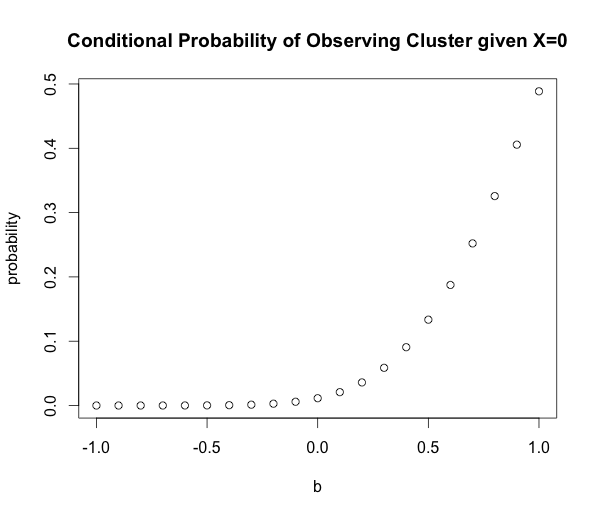
\includegraphics[scale=0.4]{Rplot1}
	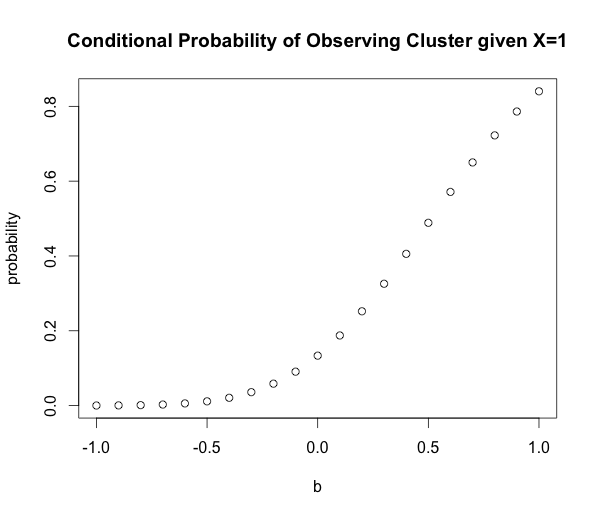
\includegraphics[scale=0.4]{Rplot2}	
\end{figure}
Viewing the graphs separately, the censoring is done in such a way that we more frequently see clusters with positive $b_i\sim N(0,1)$, which affects our intercept. Focusing on a particular value of $b_i$, the graphs also display that censoring affects the relative proportions of clusters with $X=0$ and $X=1$ instead of the mechanism which said $X=0$ and $X=1$ should occur with equal probabilities.
			\item For the multiple imputation, I set $n=10^4$ and $K=20$. Following slide 2.147, I fit two simple linear regressions. The first linear regression I fit, $Y_{i2}\sim Y_{i1}*X$, is based on observed outcomes $Y_{i2}$ on outcomes at time $t=1$ and covariate $X$ and any possible interaction, accounting for the fact that I want the imputation of time $t=2$ to be affected by previous values $Y_{i1}$ and covariate values $X_i$ and any possible interaction. \\ \\The second linear regression is based on observed outcomes $Y_{i3}\sim Y_{i2}*Y_{i1}*X$ on observed outcomes at times $t=1,2$ and covariate $X$, again including interaction terms. This is also based on the fact that when I impute observations at the third time point, I want to impute them in such a way that accounts for previous observed values at $t=1,t=2$ and covariate values $X$, again including interactions. I obtain coefficient estimates and an estimate of the variance $\widehat{\sigma}^2$ for each of the simple linear regressions. Following slide 2.157, I reflect the uncertainty in the imputation parameters just obtained by sampling new parameters based off these linear regressions via the approximate distributions $N(\widehat{\beta},\widehat{\Var}(\widehat{\beta}))$. \\ \\
		After initializing these imputation parameters, I generate new data $Y_{i2}$ as normal random variables with means centered at predicted values based on the first linear regression and variances based on our estimates of $\widehat{\sigma}$ from the linear regressions. After obtaining these imputed data, I perform these same steps above for the missing data at time $t=3$. I fit the GEE on the imputed data and repeat this $K$ times, using Rubin's rule through the MItools package in R. Mimicking my work in 1(a), I perform these steps 100 separate times and produce histograms of coefficient estimates from imputations on 100 data sets generated from this mechanism with clusters of size $n=10^4$. The histograms are
			\begin{figure}[H]
				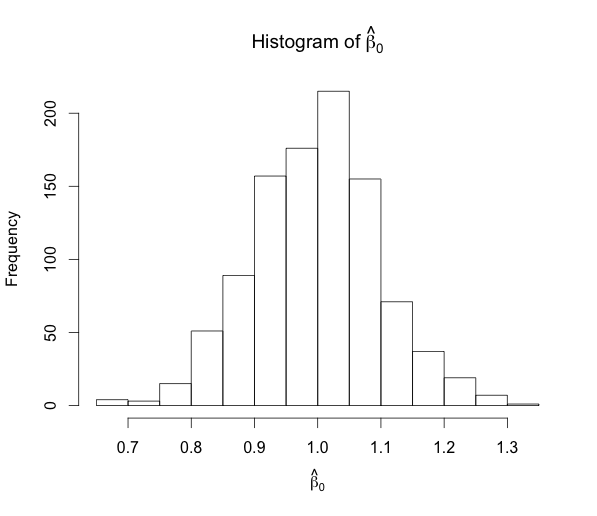
\includegraphics[scale=0.4]{Rplot1c1}
				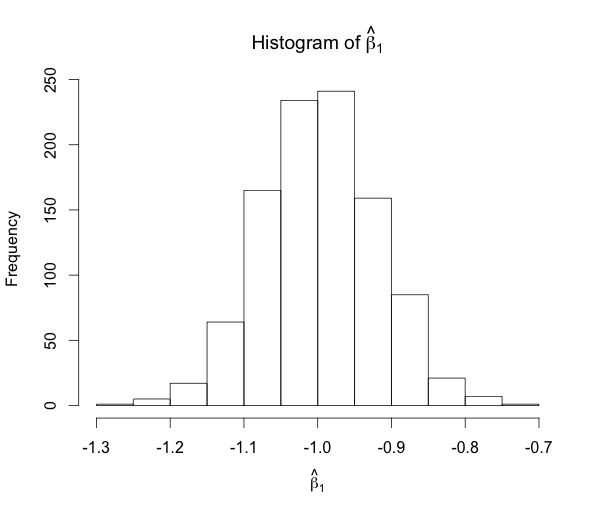
\includegraphics[scale=0.4]{Rplot1c2}
				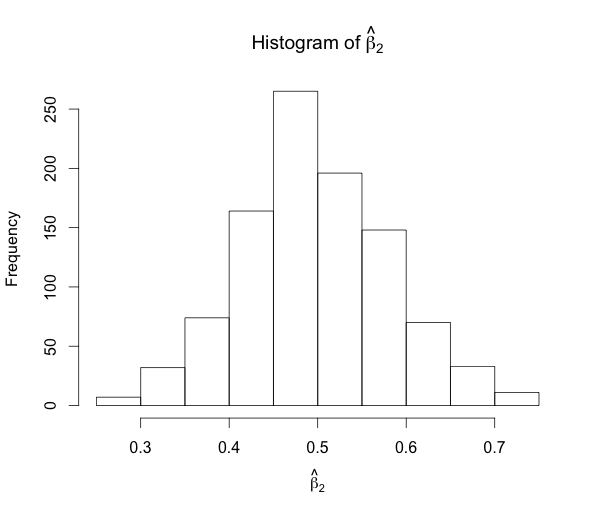
\includegraphics[scale=0.4]{Rplot1c3}
			\end{figure}
			and coverage probabilities for $\beta_0, \beta_1$ and $\beta_2$ are $27\%, 10\%, 41\%$ respectively. I am not sure if we were supposed to recover nominal coverage, though. A typical output from one of the multiple imputations with $K=20$ is
			\begin{table}[H]
			\centering
			\begin{tabular}{l|c|c|c|c|}
				              & Imputed Coefficients	 &  Imputed Standard Errors & Full Data Coefficient & Full Data SE \\
				              \hline
(Intercept)  & 1.0988752& 0.01660314 & 1.0006652 & 0.01629779\\
t          & -1.1062370 &0.00441074 & -0.9986109 & 0.00352838 \\
X          &  0.5601348 &0.02322943 & 0.4893745 & 0.02083010\\
			\end{tabular}
			\end{table}
		\end{enumerate}
	
	%2
	\item The estimate of $\widehat{\beta}_0$ is found by solving
	\[
		\frac{1}{n}\sum_{i=1}^n X_i^T V_i^{-1} \mathrm{diag}(V_{ij}^{-1})(\bm{Y}_i-\bm{\mu}_i) = 0,
	\]
	where $V_i = \phi\begin{pmatrix}
		1 & \alpha \\ \alpha & 1
	\end{pmatrix}$ and $\bm{\mu}_i = \begin{pmatrix}
		\beta_0 \\ \beta_0
	\end{pmatrix}$ so that $V_{ij} = \phi$ and $X_i = \begin{pmatrix}
		1 \\ 1
	\end{pmatrix}$. We therefore solve
	\[
		\frac{1}{n\phi^2(1-\alpha^2)}\sum_{i=1}^n \begin{pmatrix}
			1 & 1
		\end{pmatrix}\begin{pmatrix}
			1 & -\alpha \\ -\alpha & 1
		\end{pmatrix}\begin{pmatrix}
			Y_{i1} - \beta_0 \\ Y_{i2} - \beta_0
		\end{pmatrix} = 0,
	\]
	which simplifies to
	\[
		\frac{1-\alpha}{n\phi^2(1-\alpha^2)}\sum_{i=1}^n (Y_{i1}+Y_{i2}-2\beta_0) = 0\Longrightarrow \widehat{\beta}_0 = \frac{1}{2n}\sum_{i=1}^n Y_{i1} + Y_{i2}. 
	\]
	The expectations are
	\begin{align*}
		E[\widehat{\beta}_0] &= \frac{1}{2n}E\left[\sum_{i=1}^n Y_{i1}+Y_{i2}\right] \\
		&= \frac{1}{2n}E\left[E\left[\sum_{i=1}^n Y_{i1}+Y_{i2} | b_i\right]\right] \\
		&= \frac{1}{2n}E\left[\sum_{i=1}^n 2\beta_0 + 2b_i \right] \\
		&= \beta_0,
	\end{align*}
	where we use the fact that $E[b_i] = 0$ to conclude that $\widehat{\beta}_0$ is unbiased for the parameter $\beta_0$ and hence consistent by the law of large numbers since the variables $\frac{Y_{i1}+Y_{i2}}{2}, i=1,2,\dotsc$ are uncorrelated. We can also just argue that estimates found from solving the GEE are consistent for the true parameter if the mean model is correct, which relies on $E[b_i] = 0$.
	\\ \\ Since we have a balanced design, the inverse-variance weighting in the GEE does not have an affect on any of the other estimates obtained from earlier work, so we can use the estimates on slide 3.13, which are given by
	\begin{align*}
		\widehat{\sigma}^2_b &= \frac{1}{2n}\sum_{i=1}^n (Y_{i1}-\widehat{\beta}_0)(Y_{i2}-\widehat{\beta}_0) \\
		\widehat{\sigma}^2_Y &= \frac{1}{2n}\sum_{i=1}^n(Y_{i1}-\widehat{\beta}_0)^2+(Y_{i2} - \widehat{\beta}_0)^2 - \widehat{\sigma}^2_b \\
		\widehat{\alpha} &= \frac{\widehat{\sigma}^2_b}{\widehat{\sigma}^2_b+\widehat{\sigma}^2_Y}.
	\end{align*}
	Under the hypotheses in the problem, we've already noted that we have $E[Y_{ij}|X_i] = \beta_0$. For $i,i',j,j'$, we have
	\begin{align*}
		\Cov(Y_{ij},Y_{i'j'}) &= \Cov(\beta_0 + b_i + \epsilon_{ij}, \beta_0 + b_{i'} + \epsilon_{i'j'}) \\
		&= \Cov(b_i + \epsilon_{ij}, \beta_{i'} + \epsilon_{i'j'}) \\
		&= \Cov(b_i,b_{i'}) + \Cov(b_i,\epsilon_{i'j'}) + \Cov(\epsilon_{ij},b_{i'}) + \Cov(\epsilon_{ij},\epsilon_{i'j'})\\
		&= \Cov(b_i,b_{i'})+ \Cov(\epsilon_{ij},\epsilon_{i'j'}).
		\end{align*}
		If $i\neq i'$, then the covariance is zero under our model. If we are within a cluster, the intra-cluster covariance is $\Cov(Y_{ij},Y_{ij'}) = \sigma^2_b$ and the variance of observations is $\Var(Y_{ij}) = \sigma^2_b + \sigma^2_Y$.\\
	
	These three estimates given above are therefore consistent for $\sigma^2_b, \sigma^2_Y, $ and $\alpha$ provided it is actually the case that the marginal model is true as in GEE last chapter (slide 3.12). To answer the question then, if the marginal model is correct, we have $\widehat{\beta}_0$ consistent for $\beta_0$, we have $\widehat{\sigma}_Y^2$ consistent for $\sigma^2_Y = \phi(1-\alpha)$ and $\widehat{\alpha}$ consistent for the intra-cluster correlation $\alpha = \frac{\sigma^2_b}{\sigma^2_b + \sigma^2_Y}$.
	\\ \\ In the Neyman Scott problem, however, we have separate intra-cluster means $\mu_i$ and a grand variance $\tau^2$, where \emph{all} observations are independent. If we want consistency under the Neyman-Scott model, we would need to know that the true intra-cluster covariance is zero, which gives $\sigma^2_b = \alpha = 0$ and thus $b_i \equiv 0$ for all $i$.
\newpage
	\begin{align*}
		E[\widehat{\sigma}_b^2] &= \frac{1}{2n}\sum_{i=1}^n E[(Y_{i1}-\widehat{\beta}_0)(Y_{i2}-\widehat{\beta}_0)] \\
		&= \frac{1}{2n}\sum_{i=1}^n (E[Y_{i1}Y_{i2}]-E[Y_{i1}\widehat{\beta}_0]-E[Y_{i2}\widehat{\beta}_0] + E[\widehat{\beta}_0^2])
	\end{align*}
	To handle these terms, we rely on the independence assumptions, which allows us to write $E[Y_{ij}Y_{i'j'}] = E[Y_{ij}]E[Y_{i'j'}]$ so long as $i\neq i'$. The first term $E[Y_{i1}Y_{i2}] = E[Y_{i1}]E[Y_{i2}] + \Cov(Y_{i1},Y_{i2}) = \beta_0^2 + \sigma^2_b$ from previous calculation and from the derivation in class. The quantity
	\begin{align*}
		E[Y_{i1}\widehat{\beta}_0] &= \frac{1}{2n}E\left[Y_{i1}\left(\sum_{j=1}^n Y_{j1}+Y_{j2} \right)\right] \\
		&= \frac{1}{2n}\left(\left\{\sum_{j\neq i} E[Y_{i1}]E[Y_{j1}] + E[Y_{i1}]E[Y_{j2}]\right\} + E[Y_{i1}^2] + E[Y_{i1}Y_{i2}]\right) \\
		&= \frac{1}{2n}(2(n-1)\beta_0^2 + \sigma^2_Y + \sigma^2_b + \beta_0^2 + \beta_0^2 + \sigma^2_b) \\
		&= \beta_0^2 + \frac{1}{n} \sigma^2_b + \frac{1}{2n}\sigma^2_Y
	\end{align*}
	and similarly,
	\begin{align*}
		E[Y_{i2}\widehat{\beta}_0] &= \frac{1}{2n}E\left[Y_{i2}\left(\sum_{j=1}^n Y_{j1}+Y_{j2} \right)\right] \\
		&= \frac{1}{2n}\left(\left\{\sum_{j\neq i} E[Y_{i2}]E[Y_{j1}] + E[Y_{i2}]E[Y_{j2}]\right\} + E[Y_{i2}^2] + E[Y_{i2}Y_{i1}]\right) \\
		&= \frac{1}{2n}(2(n-1)\beta_0^2 + \sigma^2_Y + \sigma^2_b + \beta_0^2 + \beta_0^2 + \sigma^2_b) \\
		&= \beta_0^2 + \frac{1}{n} \sigma^2_b + \frac{1}{2n}\sigma^2_Y
	\end{align*}
	The very last term is found through the variance of $\widehat{\beta}_0$:
	\begin{align*}
		\Var(\widehat{\beta}_0) &= \frac{1}{4n^2} \sum_{i=1}^n[\Var(Y_{i1}) + \Var(Y_{i2}) + 2\Cov(Y_{i1},Y_{i2})] \\
		&= \frac{n(2(\sigma^2_Y + \sigma^2_b)+2\sigma^2_b)}{4n^2} \\
		&= \frac{\sigma^2_Y + 2\sigma^2_b}{2n} \\
		&= \frac{1}{n}\sigma^2_b + \frac{1}{2n}\sigma^2_Y
	\end{align*}
	so that $E[\widehat{\beta}_0^2] = \beta_0^2 + \frac{1}{n}\sigma^2_b + \frac{1}{2n}\sigma^2_Y $. Plugging all this in, we have
	\[
		E[\widehat{\sigma}_b^2] = \frac{1}{2n}\sum_{i=1}^n \beta_0^2 + \sigma^2_b - (\beta_0^2 + \frac{1}{n}\sigma^2_b + \frac{1}{2n}\sigma^2_Y) = \frac{n-1}{n}\sigma^2_b - \frac{1}{2n}\sigma^2_Y.
	\]	
	This is really strange because I think this quantity can be negative, so our estimate of a positive quantity does not seem that great. However, the algebra works out. We next find
	\begin{align*}
		E[\widehat{\sigma}_Y^2 + \widehat{\sigma}^2_b] &= \frac{1}{2n}\sum_{i=1}^n E[(Y_{i1}-\widehat{\beta}_0)^2] + E[(Y_{i2}-\widehat{\beta}_0)^2] 
		\\ 
		&= \frac{1}{2n}(2n)(\sigma^2_b + \sigma^2_Y + \beta_0^2 - \beta_0^2 - \frac{1}{n}\sigma^2_b - \frac{1}{2n}\sigma^2_Y) \\
		&= \frac{n-1}{n}\sigma^2_b + \frac{2n-1}{2n}\sigma^2_Y,
	\end{align*}
	so that
	\[
		E[\widehat{\sigma}^2_Y] = \frac{n-1}{n}\sigma^2_b + \frac{2n-1}{2n}\sigma^2_Y - \left[\frac{n-1}{n}\sigma^2_b - \frac{1}{2n}\sigma^2_Y\right] = \sigma^2_Y,
	\]
	so $\widehat{\sigma}^2_Y$ is a consistent estimator of its mean. The estimate
	\[
		\widehat{\alpha} = \frac{\widehat{\sigma}^2_b}{\widehat{\sigma}^2_b + \widehat{\sigma}^2_Y},
	\]
	and since the numerator has expectation $E[\widehat{\sigma}_b^2] = \frac{n-1}{n}\sigma^2_b - \frac{1}{2n}\sigma^2_Y$ and denominator has expectation $E[\widehat{\sigma}^2_b + \widehat{\sigma}^2_Y]= \frac{n-1}{n}\sigma^2_b + \frac{2n-1}{2n}\sigma^2_Y$, as $n\to\infty$, we have
	\[
		E[\widehat{\sigma}^2_b] \to \sigma^2_b,\quad E[\widehat{\sigma}^2_b + \widehat{\sigma}^2_Y] \to \sigma^2_b + \sigma^2_Y.
	\]
	Since both estimators are averages of random variables, the law of large numbers gives $\widehat{\sigma}^2_b \to_p \sigma^2_b$ and $\widehat{\sigma}^2_b + \widehat{\sigma}^2_Y \to_p \sigma^2_b + \sigma^2_Y$, and by Slutsky's theorem, we finally have $\widehat{\alpha} \to_p \frac{\sigma^2_b}{\sigma^2_b + \sigma^2_Y}$, the intra-cluster correlation.
	\end{enumerate}
	\newpage
	\begin{verbatim}
		library(geeM)
library(gee)
library(reshape2)
library(ggplot2)
library(mitools)
#p1
set.seed(571)
sb = 1
sy = 0.5
beta0 = 1
beta1 = -1
beta2 = 0.5
n = 10^3
betas = matrix(0,nrow=10^3,ncol=3)
count0 = 0
count1 = 0
count2 = 0
for(k in 1:10^3)
{
  b = rnorm(n,mean=0,sd=sb)
  X = rbinom(n,1,0.5)
  y = c()
  for(i in 1:n)
  {
    mu = beta0 + b[i] + beta1*(1:3) + beta2*X[i] 
    y = append(y,rnorm(3, mean = mu, sd = sy))
  }
  dat = data.frame(Y = y,X = rep(X,each=3),t = rep(1:3,n),id = rep(1:n,each=3))
  missing = dat
  inds = 3*(0:(n-1))+1
  for(i in inds)
  {
    for(j in 0:1)
    {
      if(dat$Y[i+j] < 0)
      {
        missing$Y[((i+j+1):(i+2))] <- NA
        break
      }
    }
  }
  model = geem(Y~t+X,id=id,data=dat,corstr="independence")
  model3 = geem(Y~t+X,id=id,data=missing,corstr="independence")
  betas[k,] = model3$beta
  len = 1.96*summary(model3)$se.robust
  if(
    findInterval(beta0,model3$beta[1] + c(-1,1)*len[1]) == 1
  )
  {
    count0 = count0 + 1
  }
  if(
    findInterval(beta1,model3$beta[2] + c(-1,1)*len[2]) == 1
  )
  {
    count1 = count1 + 1
  }
  if(
    findInterval(beta2,model3$beta[3] + c(-1,1)*len[3]) == 1
  )
  {
    count2 = count2 + 1
  }
}
hist(betas[,1],main=expression(paste("Histogram of ", hat(beta)[0])),xlab=expression(hat(beta)[0]))
hist(betas[,2],main=expression(paste("Histogram of ", hat(beta)[1])),xlab=expression(hat(beta)[1]))
hist(betas[,3],main=expression(paste("Histogram of ", hat(beta)[2])),xlab=expression(hat(beta)[2]))
hists = melt(data.frame(cbind(1:10^3,betas)),'X1')
ggplot(hists, aes(x=value)) + geom_histogram(binwidth=0.1) + facet_wrap(~variable)
ggplot(m,aes(value)) + geom_bar(binwidth = 1) + facet_wrap(~variable)
# > count0
# [1] 0
# > count1
# [1] 0
# > count2
# [1] 485
#1b
censor <- function(x,b)
{
  return(
    pnorm((-b-0.5*x)/0.5) + pnorm((-b-0.5*x+1)/0.5) - pnorm((-b-0.5*x)/0.5)*pnorm((-b-0.5*x+1)/0.5)
  )
}
b = seq(-1,1,0.1)
plot(b,1-censor(0,b),main="Conditional Probability of Observing Cluster given X=0",ylab="probability")
plot(b,1-censor(1,b),main="Conditional Probability of Observing Cluster given X=1", ylab="probability")

hist(subset(missing,t==1)$Y)
hist(subset(missing,t==2)$Y)
hist(subset(missing,t==3)$Y)

##1c
n = 10^2
count0 = 0
count1 = 0
count2 = 0
NEWbetas = matrix(0,nrow=1,ncol=3)
for(m in 1)
{
  b = rnorm(n,mean=0,sd=sb)
  X = rbinom(n,1,0.5)
  y = c()
  for(i in 1:n)
  {
    mu = beta0 + b[i] + beta1*(1:3) + beta2*X[i] 
    y = append(y,rnorm(3, mean = mu, sd = sy))
  }
  dat = data.frame(Y = y,X = rep(X,each=3),t = rep(1:3,n),id = rep(1:n,each=3))
  missing = dat
  inds = 3*(0:(n-1))+1
  temp = c()
  for(i in inds)
  {
    for(j in 0:1)
    {
      if(dat$Y[i+j] < 0)
      {
        missing$Y[((i+j+1):(i+2))] <- NA
        break
      }
    }
  }
  model = gee(Y~t+X,id=id,data=dat,corstr="independence")
  model2 = gee(Y~t+X,id=id,data=missing,corstr="independence")
  
  #focus on missing DF
  time1 = subset(missing,t==1)
  miss2 = is.na(missing$Y) & missing$t==2
  miss3 = is.na(missing$Y) & missing$t==3
  clusters = missing[miss2,4] #CLUSTERS MISSING A TIME 2 INDEX
  firstImpY = subset(missing,t==2)$Y
  a = subset(missing,id%in%clusters & t==1) #used for prediction
  mod2 <- lm(firstImpY ~ Y*X, data=time1)
  secondImpY = subset(missing,t==3)$Y
  first2 = subset(missing, t!=3)
  wide = reshape(first2,timevar="t", idvar=c("X","id"),direction="wide")
  mod3 <- lm(secondImpY~Y.1*Y.2*X, data=wide)
  param2 = rnorm(4,mean=summary(mod2)$coefficients[,1],sd=summary(mod2)$coefficients[,2])
  mod2$coefficients = param2
  
  
  param3 = rnorm(8,mean=summary(mod3)$coefficients[,1],sd=summary(mod3)$coefficients[,2])
  mod3$coefficients = param3
  
  sig2 = sqrt(summary(mod2)$sigma^2*rchisq(1,mod2$df.residual)/mod2$df.residual)
  sig3 = sqrt(summary(mod3)$sigma^2*rchisq(1,mod3$df.residual)/mod3$df.residual)
  
  do.one <- function(n)
  {
    miss.i <- missing
  
    mu2 = predict(mod2,a[,-c(3,4)]);
    miss.i[ miss2, "Y"] <- rnorm( sum( miss2), mu2, summary(mod2)$sigma )
    
    
    clusters3 = miss.i[miss3,4]
    b = subset(miss.i,id%in%clusters3 & t!=3)
    blah = reshape(b,timevar="t", idvar=c("X", "id"),direction="wide")
    blah = blah[-2]
    mu3 = predict(mod3,blah);
    
    miss.i[miss3, "Y"] <- rnorm(sum(miss3), mu3, summary(mod3)$sigma)
    
    gee.i <- gee(Y~t+X, id=id,
                  data=miss.i, corstr="independence")
    gee.i
  }
  
  my.mi <- replicate(20, do.one(), simplify=FALSE)
  betas <- MIextract(my.mi, fun=coef)
  vars <- MIextract(my.mi, fun=function(x){as.matrix(x$robust.variance)})
  imputed = MIcombine(betas,vars)
  low = summary(imputed)$`(lower`
  up = summary(imputed)$`upper)`
  NEWbetas[m,] = imputed$coefficients
  if( findInterval(beta0,rbind(low,up)[,1]) == 1)
  {
    count0 = count0 + 1
  }
  if( findInterval(beta1,rbind(low,up)[,2]) == 1)
  {
    count1 = count1 + 1
  }
  if( findInterval(beta2,rbind(low,up)[,3]) == 1)
  {
    count2 = count2 + 1
  }
}

coplot(Y~t|factor(id),data=missing,show.given=F,
       panel=function(x,y,col,...){points(x,y,col=col)
         lines(x,y,col=col)})

matplot(missing$t,missing$Y,type="l",lty=1,
         xlab="time", ylab="Observation", main="Spaghetti Plot of Observations")

mine = NEWbetas[1:1000,]
hist(mine[,1],main=expression(paste("Histogram of ", hat(beta)[0])),xlab=expression(hat(beta)[0]))
hist(mine[,2],main=expression(paste("Histogram of ", hat(beta)[1])),xlab=expression(hat(beta)[1]))
hist(mine[,3],main=expression(paste("Histogram of ", hat(beta)[2])),xlab=expression(hat(beta)[2]))

	\end{verbatim}
\end{document}



